% Options for packages loaded elsewhere
\PassOptionsToPackage{unicode}{hyperref}
\PassOptionsToPackage{hyphens}{url}
\PassOptionsToPackage{dvipsnames,svgnames,x11names}{xcolor}
%
\documentclass[
  letterpaper,
  DIV=11,
  numbers=noendperiod]{scrartcl}

\usepackage{amsmath,amssymb}
\usepackage{iftex}
\ifPDFTeX
  \usepackage[T1]{fontenc}
  \usepackage[utf8]{inputenc}
  \usepackage{textcomp} % provide euro and other symbols
\else % if luatex or xetex
  \usepackage{unicode-math}
  \defaultfontfeatures{Scale=MatchLowercase}
  \defaultfontfeatures[\rmfamily]{Ligatures=TeX,Scale=1}
\fi
\usepackage{lmodern}
\ifPDFTeX\else  
    % xetex/luatex font selection
\fi
% Use upquote if available, for straight quotes in verbatim environments
\IfFileExists{upquote.sty}{\usepackage{upquote}}{}
\IfFileExists{microtype.sty}{% use microtype if available
  \usepackage[]{microtype}
  \UseMicrotypeSet[protrusion]{basicmath} % disable protrusion for tt fonts
}{}
\makeatletter
\@ifundefined{KOMAClassName}{% if non-KOMA class
  \IfFileExists{parskip.sty}{%
    \usepackage{parskip}
  }{% else
    \setlength{\parindent}{0pt}
    \setlength{\parskip}{6pt plus 2pt minus 1pt}}
}{% if KOMA class
  \KOMAoptions{parskip=half}}
\makeatother
\usepackage{xcolor}
\setlength{\emergencystretch}{3em} % prevent overfull lines
\setcounter{secnumdepth}{-\maxdimen} % remove section numbering
% Make \paragraph and \subparagraph free-standing
\ifx\paragraph\undefined\else
  \let\oldparagraph\paragraph
  \renewcommand{\paragraph}[1]{\oldparagraph{#1}\mbox{}}
\fi
\ifx\subparagraph\undefined\else
  \let\oldsubparagraph\subparagraph
  \renewcommand{\subparagraph}[1]{\oldsubparagraph{#1}\mbox{}}
\fi

\usepackage{color}
\usepackage{fancyvrb}
\newcommand{\VerbBar}{|}
\newcommand{\VERB}{\Verb[commandchars=\\\{\}]}
\DefineVerbatimEnvironment{Highlighting}{Verbatim}{commandchars=\\\{\}}
% Add ',fontsize=\small' for more characters per line
\newenvironment{Shaded}{}{}
\newcommand{\AlertTok}[1]{\textcolor[rgb]{1.00,0.33,0.33}{\textbf{#1}}}
\newcommand{\AnnotationTok}[1]{\textcolor[rgb]{0.42,0.45,0.49}{#1}}
\newcommand{\AttributeTok}[1]{\textcolor[rgb]{0.84,0.23,0.29}{#1}}
\newcommand{\BaseNTok}[1]{\textcolor[rgb]{0.00,0.36,0.77}{#1}}
\newcommand{\BuiltInTok}[1]{\textcolor[rgb]{0.84,0.23,0.29}{#1}}
\newcommand{\CharTok}[1]{\textcolor[rgb]{0.01,0.18,0.38}{#1}}
\newcommand{\CommentTok}[1]{\textcolor[rgb]{0.42,0.45,0.49}{#1}}
\newcommand{\CommentVarTok}[1]{\textcolor[rgb]{0.42,0.45,0.49}{#1}}
\newcommand{\ConstantTok}[1]{\textcolor[rgb]{0.00,0.36,0.77}{#1}}
\newcommand{\ControlFlowTok}[1]{\textcolor[rgb]{0.84,0.23,0.29}{#1}}
\newcommand{\DataTypeTok}[1]{\textcolor[rgb]{0.84,0.23,0.29}{#1}}
\newcommand{\DecValTok}[1]{\textcolor[rgb]{0.00,0.36,0.77}{#1}}
\newcommand{\DocumentationTok}[1]{\textcolor[rgb]{0.42,0.45,0.49}{#1}}
\newcommand{\ErrorTok}[1]{\textcolor[rgb]{1.00,0.33,0.33}{\underline{#1}}}
\newcommand{\ExtensionTok}[1]{\textcolor[rgb]{0.84,0.23,0.29}{\textbf{#1}}}
\newcommand{\FloatTok}[1]{\textcolor[rgb]{0.00,0.36,0.77}{#1}}
\newcommand{\FunctionTok}[1]{\textcolor[rgb]{0.44,0.26,0.76}{#1}}
\newcommand{\ImportTok}[1]{\textcolor[rgb]{0.01,0.18,0.38}{#1}}
\newcommand{\InformationTok}[1]{\textcolor[rgb]{0.42,0.45,0.49}{#1}}
\newcommand{\KeywordTok}[1]{\textcolor[rgb]{0.84,0.23,0.29}{#1}}
\newcommand{\NormalTok}[1]{\textcolor[rgb]{0.14,0.16,0.18}{#1}}
\newcommand{\OperatorTok}[1]{\textcolor[rgb]{0.14,0.16,0.18}{#1}}
\newcommand{\OtherTok}[1]{\textcolor[rgb]{0.44,0.26,0.76}{#1}}
\newcommand{\PreprocessorTok}[1]{\textcolor[rgb]{0.84,0.23,0.29}{#1}}
\newcommand{\RegionMarkerTok}[1]{\textcolor[rgb]{0.42,0.45,0.49}{#1}}
\newcommand{\SpecialCharTok}[1]{\textcolor[rgb]{0.00,0.36,0.77}{#1}}
\newcommand{\SpecialStringTok}[1]{\textcolor[rgb]{0.01,0.18,0.38}{#1}}
\newcommand{\StringTok}[1]{\textcolor[rgb]{0.01,0.18,0.38}{#1}}
\newcommand{\VariableTok}[1]{\textcolor[rgb]{0.89,0.38,0.04}{#1}}
\newcommand{\VerbatimStringTok}[1]{\textcolor[rgb]{0.01,0.18,0.38}{#1}}
\newcommand{\WarningTok}[1]{\textcolor[rgb]{1.00,0.33,0.33}{#1}}

\providecommand{\tightlist}{%
  \setlength{\itemsep}{0pt}\setlength{\parskip}{0pt}}\usepackage{longtable,booktabs,array}
\usepackage{calc} % for calculating minipage widths
% Correct order of tables after \paragraph or \subparagraph
\usepackage{etoolbox}
\makeatletter
\patchcmd\longtable{\par}{\if@noskipsec\mbox{}\fi\par}{}{}
\makeatother
% Allow footnotes in longtable head/foot
\IfFileExists{footnotehyper.sty}{\usepackage{footnotehyper}}{\usepackage{footnote}}
\makesavenoteenv{longtable}
\usepackage{graphicx}
\makeatletter
\def\maxwidth{\ifdim\Gin@nat@width>\linewidth\linewidth\else\Gin@nat@width\fi}
\def\maxheight{\ifdim\Gin@nat@height>\textheight\textheight\else\Gin@nat@height\fi}
\makeatother
% Scale images if necessary, so that they will not overflow the page
% margins by default, and it is still possible to overwrite the defaults
% using explicit options in \includegraphics[width, height, ...]{}
\setkeys{Gin}{width=\maxwidth,height=\maxheight,keepaspectratio}
% Set default figure placement to htbp
\makeatletter
\def\fps@figure{htbp}
\makeatother

\KOMAoption{captions}{tableheading,figureheading}
\makeatletter
\makeatother
\makeatletter
\makeatother
\makeatletter
\@ifpackageloaded{caption}{}{\usepackage{caption}}
\AtBeginDocument{%
\ifdefined\contentsname
  \renewcommand*\contentsname{Tabla de contenidos}
\else
  \newcommand\contentsname{Tabla de contenidos}
\fi
\ifdefined\listfigurename
  \renewcommand*\listfigurename{Listado de Figuras}
\else
  \newcommand\listfigurename{Listado de Figuras}
\fi
\ifdefined\listtablename
  \renewcommand*\listtablename{Listado de Tablas}
\else
  \newcommand\listtablename{Listado de Tablas}
\fi
\ifdefined\figurename
  \renewcommand*\figurename{Figura}
\else
  \newcommand\figurename{Figura}
\fi
\ifdefined\tablename
  \renewcommand*\tablename{Tabla}
\else
  \newcommand\tablename{Tabla}
\fi
}
\@ifpackageloaded{float}{}{\usepackage{float}}
\floatstyle{ruled}
\@ifundefined{c@chapter}{\newfloat{codelisting}{h}{lop}}{\newfloat{codelisting}{h}{lop}[chapter]}
\floatname{codelisting}{Listado}
\newcommand*\listoflistings{\listof{codelisting}{Listado de Listados}}
\makeatother
\makeatletter
\@ifpackageloaded{caption}{}{\usepackage{caption}}
\@ifpackageloaded{subcaption}{}{\usepackage{subcaption}}
\makeatother
\makeatletter
\@ifpackageloaded{tcolorbox}{}{\usepackage[skins,breakable]{tcolorbox}}
\makeatother
\makeatletter
\@ifundefined{shadecolor}{\definecolor{shadecolor}{rgb}{.97, .97, .97}}
\makeatother
\makeatletter
\makeatother
\makeatletter
\makeatother
\ifLuaTeX
\usepackage[bidi=basic]{babel}
\else
\usepackage[bidi=default]{babel}
\fi
\babelprovide[main,import]{spanish}
% get rid of language-specific shorthands (see #6817):
\let\LanguageShortHands\languageshorthands
\def\languageshorthands#1{}
\ifLuaTeX
  \usepackage{selnolig}  % disable illegal ligatures
\fi
\usepackage[]{biblatex}
\addbibresource{../../../../references.bib}
\IfFileExists{bookmark.sty}{\usepackage{bookmark}}{\usepackage{hyperref}}
\IfFileExists{xurl.sty}{\usepackage{xurl}}{} % add URL line breaks if available
\urlstyle{same} % disable monospaced font for URLs
\hypersetup{
  pdftitle={Instalación de R en Linux},
  pdfauthor={Edison Achalma},
  pdflang={es},
  colorlinks=true,
  linkcolor={blue},
  filecolor={Maroon},
  citecolor={Blue},
  urlcolor={Blue},
  pdfcreator={LaTeX via pandoc}}

\title{Instalación de R en Linux}
\usepackage{etoolbox}
\makeatletter
\providecommand{\subtitle}[1]{% add subtitle to \maketitle
  \apptocmd{\@title}{\par {\large #1 \par}}{}{}
}
\makeatother
\subtitle{Explorando las capacidades de R y su uso en el entorno Linux}
\author{Edison Achalma}
\date{2023-06-09}

\begin{document}
\maketitle
\ifdefined\Shaded\renewenvironment{Shaded}{\begin{tcolorbox}[boxrule=0pt, interior hidden, borderline west={3pt}{0pt}{shadecolor}, breakable, frame hidden, enhanced, sharp corners]}{\end{tcolorbox}}\fi

\hypertarget{instalaciuxf3n}{%
\section{Instalación}\label{instalaciuxf3n}}

En este artículo, te guiaré para descargar e instalar R y RStudio en
sistema operativo Ubuntu Linux.

\hypertarget{paso-1.-descargar-r-en-ubuntu-linux}{%
\subsection{Paso 1. Descargar R en Ubuntu
Linux}\label{paso-1.-descargar-r-en-ubuntu-linux}}

Para comenzar, necesitarás descargar el paquete de instalación de R
desde el sitio web oficial de R. Abre tu navegador web y sigue este
enlace: \href{https://cloud.r-project.org/}{Enlace de descarga de R}

\begin{quote}
R es un lenguaje de programación ampliamente utilizado en la comunidad
estadística y de análisis de datos, y es especialmente popular entre los
científicos de datos y los investigadores.
\end{quote}

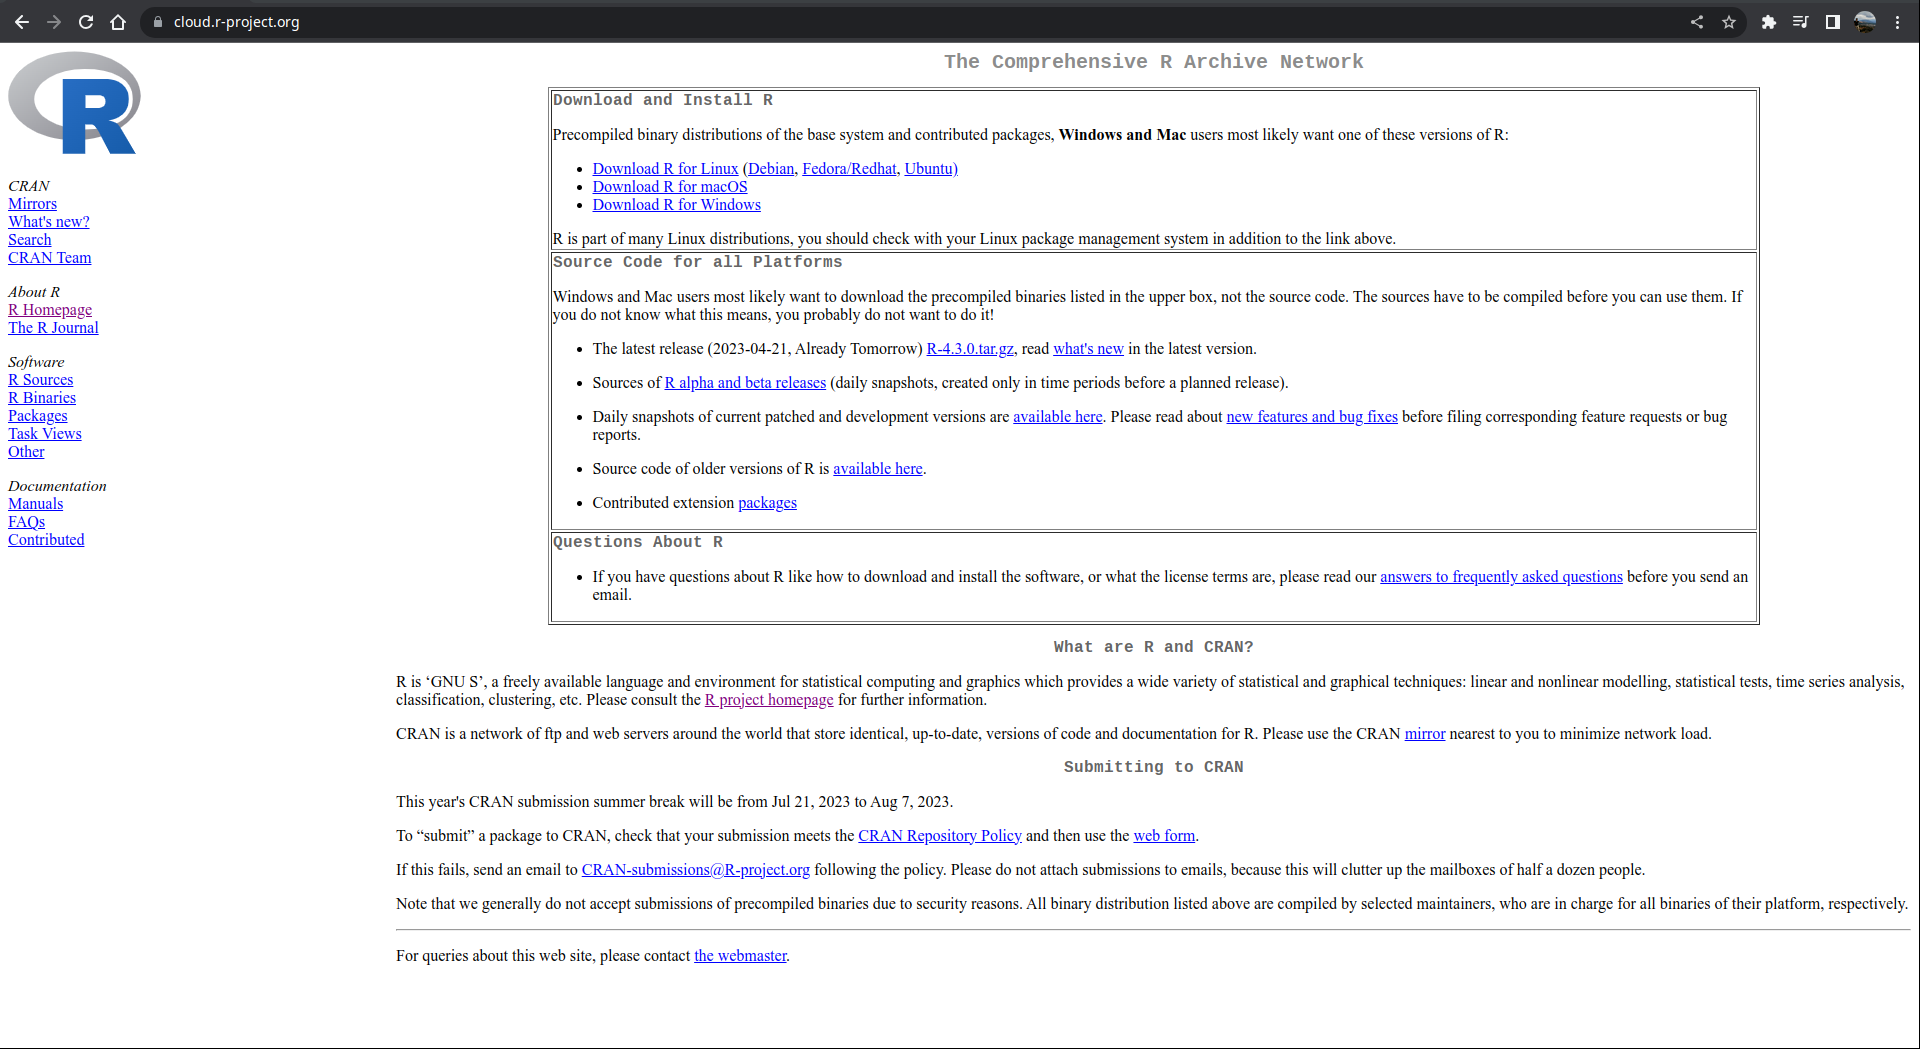
\includegraphics{images/Screenshot_20230610_222900.png}

\hypertarget{paso-2.-instalar-r-en-ubuntu-linux}{%
\subsection{Paso 2. Instalar R en Ubuntu
Linux}\label{paso-2.-instalar-r-en-ubuntu-linux}}

Los paquetes para la versión actual de R 4.2 están disponibles para la
mayoría de las versiones estables de Ubuntu Desktop. Sin embargo, solo
la última versión de Soporte a Largo Plazo (LTS) cuenta con soporte
completo. A partir del 2 de mayo de 2022, las versiones compatibles son:

\begin{itemize}
\tightlist
\item
  Jammy Jellyfish (22.04, solo amd64)
\item
  Impish Indri (21.10, solo amd64)
\item
  Focal Fossa (20.04; LTS y solo amd64)
\item
  Bionic Beaver (18.04; LTS)
\item
  Xenial Xerus (16.04; LTS)
\end{itemize}

Ejecuta estas líneas (si eres \texttt{root}, omite \texttt{sudo}) para
informar a Ubuntu sobre los binarios de R en CRAN.

\begin{Shaded}
\begin{Highlighting}[]
\CommentTok{\# Actualizar índices}
\FunctionTok{sudo}\NormalTok{ apt update }\AttributeTok{{-}qq}
\CommentTok{\# Instalar dos paquetes auxiliares necesarios}
\FunctionTok{sudo}\NormalTok{ apt install }\AttributeTok{{-}{-}no{-}install{-}recommends}\NormalTok{ software{-}properties{-}common dirmngr}
\CommentTok{\# Agregar la clave de firma (de Michael Rutter) para estos repositorios}
\CommentTok{\# Para verificar la clave, ejecuta: gpg {-}{-}show{-}keys /etc/apt/trusted.gpg.d/cran\_ubuntu\_key.asc}
\CommentTok{\# Huella digital: E298A3A825C0D65DFD57CBB651716619E084DAB9}
\FunctionTok{wget} \AttributeTok{{-}qO{-}}\NormalTok{ https://cloud.r{-}project.org/bin/linux/ubuntu/marutter\_pubkey.asc }\KeywordTok{|} \FunctionTok{sudo}\NormalTok{ tee }\AttributeTok{{-}a}\NormalTok{ /etc/apt/trusted.gpg.d/cran\_ubuntu\_key.asc}
\CommentTok{\# Agregar el repositorio de R 4.0 de CRAN {-}{-} ajustar \textquotesingle{}focal\textquotesingle{} a \textquotesingle{}groovy\textquotesingle{} o \textquotesingle{}bionic\textquotesingle{} según sea necesario}
\FunctionTok{sudo}\NormalTok{ add{-}apt{-}repository }\StringTok{"deb https://cloud.r{-}project.org/bin/linux/ubuntu }\VariableTok{$(}\ExtensionTok{lsb\_release} \AttributeTok{{-}cs}\VariableTok{)}\StringTok{{-}cran40/"}
\end{Highlighting}
\end{Shaded}

Aquí utilizamos \texttt{lsb\_release\ -cs} para acceder a la versión de
Ubuntu que estás utilizando: ``jammy'', ``impish'', ``focal'',
``bionic'', \ldots{}

Luego, ejecuta

\begin{Shaded}
\begin{Highlighting}[]
\FunctionTok{sudo}\NormalTok{ apt install }\AttributeTok{{-}{-}no{-}install{-}recommends}\NormalTok{ r{-}base}
\end{Highlighting}
\end{Shaded}

\hypertarget{obtuxe9n-muxe1s-de-5000-paquetes-de-cran}{%
\subsection{Obtén más de 5000 paquetes de
CRAN}\label{obtuxe9n-muxe1s-de-5000-paquetes-de-cran}}

Ejecuta este comando (como \texttt{root} o agregando \texttt{sudo} como
prefijo) para agregar el repositorio actual de R 4.0 o posterior
`c2d4u':

\begin{Shaded}
\begin{Highlighting}[]
\FunctionTok{sudo}\NormalTok{ add{-}apt{-}repository ppa:c2d4u.team/c2d4u4.0+}
\end{Highlighting}
\end{Shaded}

para agregar el ID de clave de este repositorio, agregar el repositorio
y actualizar el índice. Ahora puedes hacer
\texttt{apt\ install\ -\/-no-install-recommends\ r-cran-rstan} o
\texttt{apt\ install\ -\/-no-install-recommends\ r-cran-tidyverse}
(nuevamente como usuario \texttt{root} o a través de \texttt{sudo}).

\hypertarget{paso-3.-descargar-rstudio-en-ubuntu-linux}{%
\subsection{Paso 3. Descargar RStudio en Ubuntu
Linux}\label{paso-3.-descargar-rstudio-en-ubuntu-linux}}

Puedes descargar la última versión de RStudio desde su sitio web
oficial:
\href{https://www.rstudio.com/products/rstudio/download/}{Enlace de
descarga de RStudio}

\begin{quote}
RStudio RStudio es un entorno de desarrollo integrado (IDE) muy popular
para trabajar con R. Proporciona una interfaz gráfica intuitiva y muchas
herramientas útiles para la programación en R.
\end{quote}

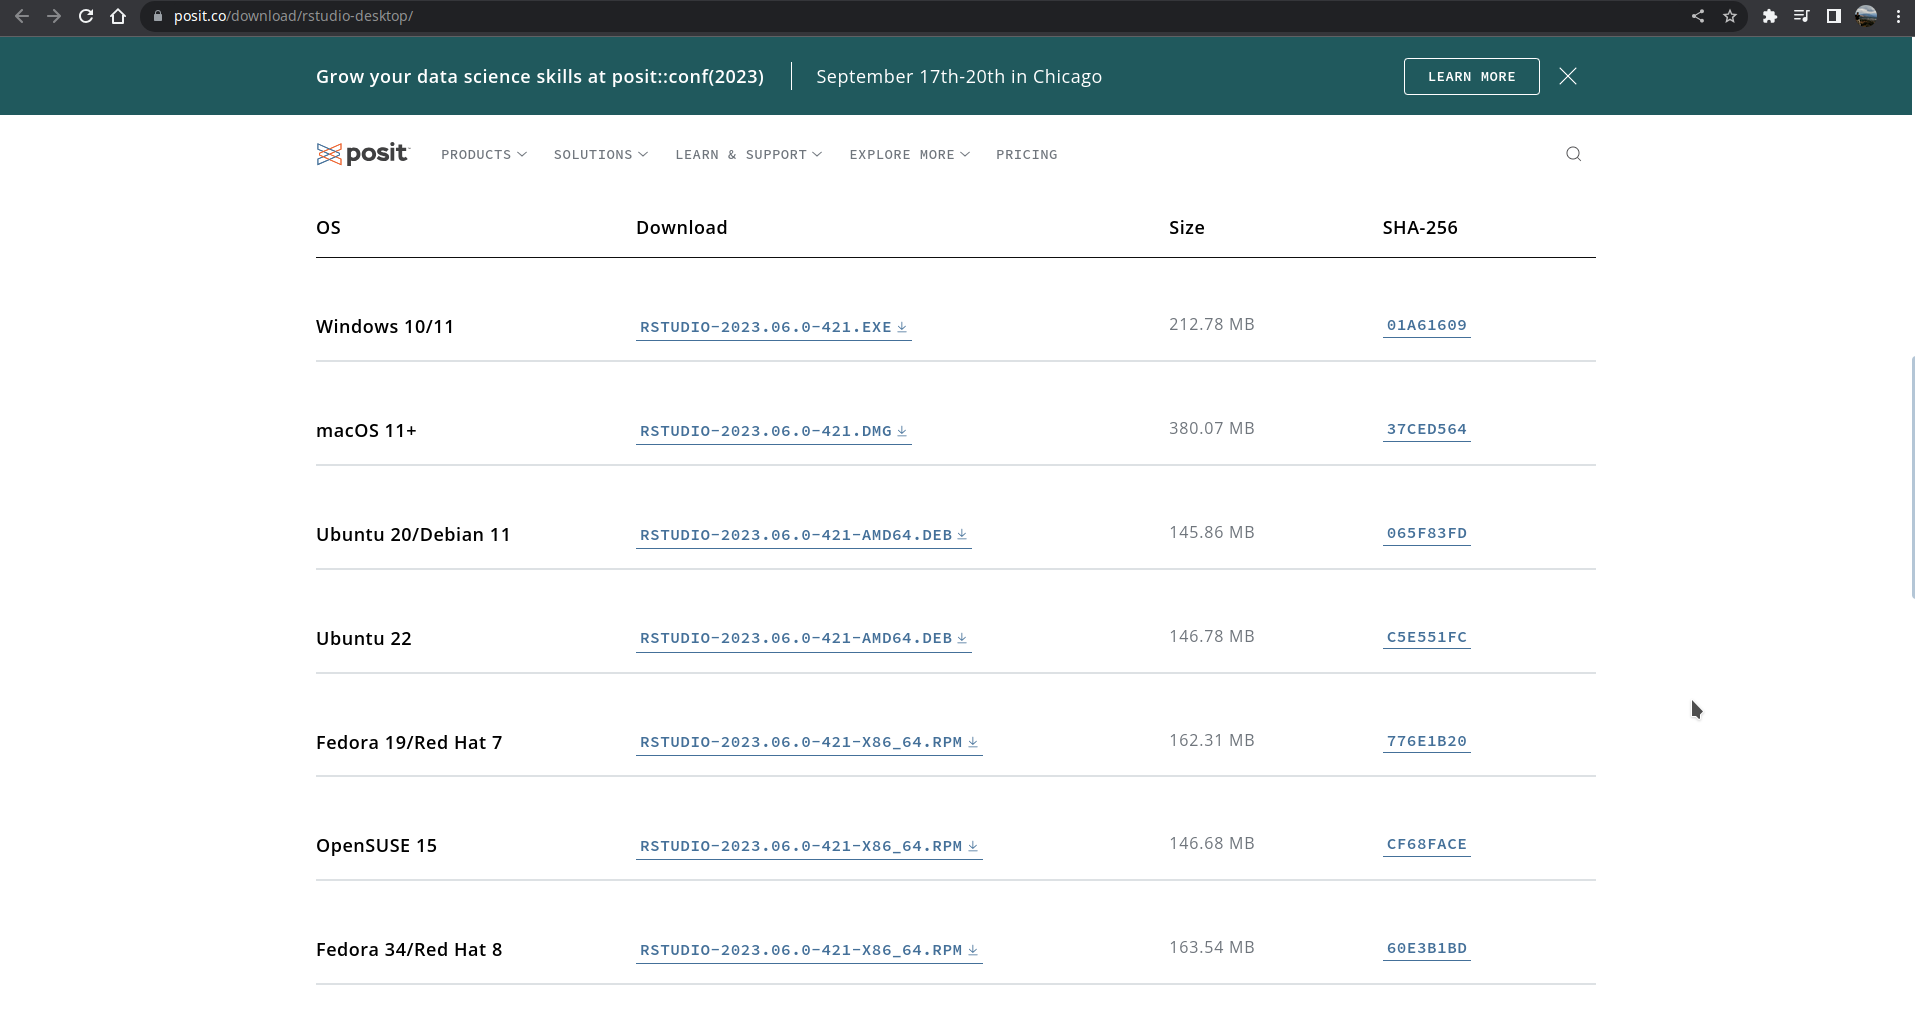
\includegraphics{images/Screenshot_20230610_224818.png}

\hypertarget{paso-4.-instalar-rstudio-en-ubuntu-linux}{%
\subsection{Paso 4. Instalar RStudio en Ubuntu
Linux}\label{paso-4.-instalar-rstudio-en-ubuntu-linux}}

\hypertarget{instalar-dependencias}{%
\subsubsection{Instalar dependencias}\label{instalar-dependencias}}

Antes de instalar RStudio, es posible que debas instalar algunas
dependencias en tu sistema. Abre la terminal y ejecuta los siguientes
comandos para instalar las dependencias requeridas:

\begin{Shaded}
\begin{Highlighting}[]
\FunctionTok{sudo}\NormalTok{ apt update}
\FunctionTok{sudo}\NormalTok{ apt install gdebi{-}core}
\end{Highlighting}
\end{Shaded}

Estos comandos actualizarán los repositorios de paquetes y luego
instalarán \texttt{gdebi-core}, una utilidad necesaria para instalar
paquetes \texttt{.deb} de forma sencilla y para resolver dependencias
automáticamente.

\hypertarget{instalar-rstudio}{%
\subsubsection{Instalar RStudio}\label{instalar-rstudio}}

Una vez que hayas descargado el archivo de instalación de RStudio y
hayas instalado las dependencias necesarias, puedes proceder con la
instalación. Ve al directorio donde descargaste el archivo de
instalación y ejecuta el siguiente comando en la terminal:

\begin{Shaded}
\begin{Highlighting}[]
\FunctionTok{sudo}\NormalTok{ gdebi }\OperatorTok{\textless{}}\NormalTok{nombre\_del\_archivo\_de\_instalación}\OperatorTok{\textgreater{}}\NormalTok{.deb}
\end{Highlighting}
\end{Shaded}

Reemplaza
\texttt{\textless{}nombre\_del\_archivo\_de\_instalación\textgreater{}}
con el nombre real del archivo de instalación descargado.

El comando \texttt{gdebi} instalará RStudio y resolverá automáticamente
las dependencias necesarias.

\hypertarget{paso-5.-iniciar-rstudio}{%
\subsection{Paso 5. Iniciar RStudio}\label{paso-5.-iniciar-rstudio}}

Una vez completada la instalación, puedes iniciar RStudio desde el menú
de aplicaciones de Ubuntu o ejecutando el siguiente comando en la
terminal:

\begin{Shaded}
\begin{Highlighting}[]
\ExtensionTok{rstudio}
\end{Highlighting}
\end{Shaded}

RStudio se abrirá en una ventana separada, lo que te permitirá comenzar
a trabajar con R y aprovechar todas las funciones y características que
ofrece el IDE.

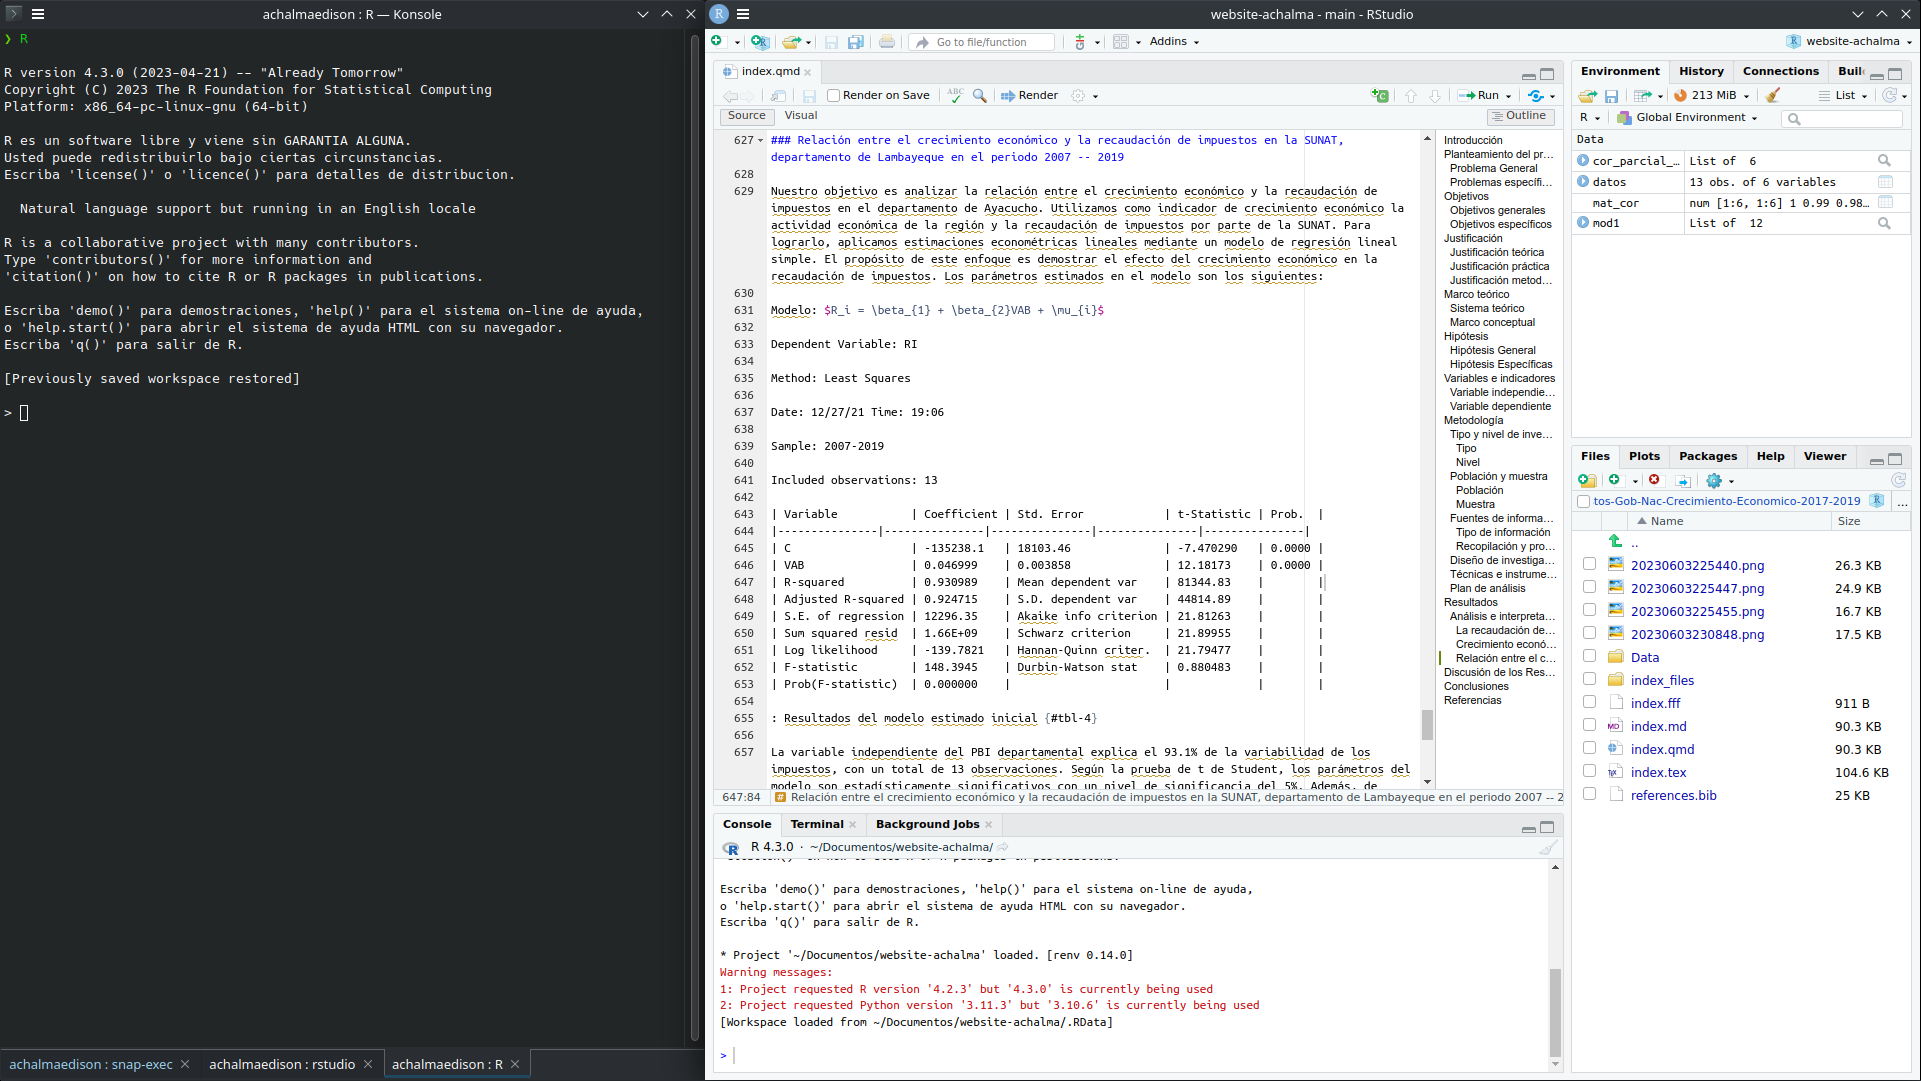
\includegraphics{images/Screenshot_20230610_231407.png}


\printbibliography


\end{document}
